\documentclass[11pt,a4paper]{article}

\usepackage[utf8]{inputenc}
\usepackage{geometry}
\geometry{a4paper, margin=1in}
\usepackage{graphicx}
\usepackage{hyperref}
\usepackage{float}
\usepackage{booktabs}
\usepackage{tcolorbox}
\usepackage{subcaption}
\usepackage{xcolor}
\usepackage{titlesec}
\usepackage{enumitem}
\usepackage{microtype} % Improves text justification and typesetting quality
\usepackage{ragged2e}  % Adds \justifying command for rigid alignment
\usepackage{setspace}  % For line spacing

% --- Custom Colors ---
\definecolor{iitjblue}{RGB}{31, 78, 121}
\definecolor{iitjgold}{RGB}{230, 159, 0}
\definecolor{highlightbg}{RGB}{245, 247, 250}
\definecolor{accentgreen}{RGB}{46, 139, 87}
\definecolor{accentred}{RGB}{205, 92, 92}

% --- Hyperlink Setup ---
\hypersetup{
    colorlinks=true,
    linkcolor=iitjblue,
    filecolor=magenta,      
    urlcolor=iitjblue,
    pdftitle={NLU Assignment 2 - Problem 1},
}

% --- Title Formatting ---
\titleformat{\section}{\Large\bfseries\color{iitjblue}}{\thesection}{1em}{}[{\titlerule[0.8pt]}]
\titleformat{\subsection}{\large\bfseries\color{iitjblue!80}}{\thesubsection}{1em}{}
\titleformat{\subsubsection}{\normalsize\bfseries\color{iitjblue!60}}{\thesubsubsection}{1em}{}

% --- Custom Boxes (Configured for Full Justification) ---
\newtcolorbox{infoBox}[1][]{
    colback=highlightbg,
    colframe=iitjblue,
    fonttitle=\bfseries,
    title=#1,
    arc=4pt,
    boxrule=1pt,
    halign=justify, % Forces justification inside the box
    left=8pt, right=8pt, top=8pt, bottom=8pt
}

\newtcolorbox{resultBox}[1][]{
    colback=green!5,
    colframe=accentgreen,
    fonttitle=\bfseries,
    title=#1,
    arc=4pt,
    boxrule=1pt,
    halign=justify, % Forces justification inside the box
    left=8pt, right=8pt, top=8pt, bottom=8pt
}

\newtcolorbox{analogyBox}[1][]{
    colback=iitjgold!10,
    colframe=iitjgold,
    fonttitle=\bfseries,
    title=#1,
    arc=4pt,
    boxrule=1pt,
    halign=justify, % Forces justification inside the box
    left=8pt, right=8pt, top=8pt, bottom=8pt
}

\title{\Huge\textbf{\color{iitjblue} NLU Assignment 2}\\[0.5em] \LARGE \color{iitjblue!80} Problem 1: Learning Word Embeddings from IIT Jodhpur Data}
\author{\Large \textbf{Arnesh Singh}}
\date{\large \today}

\begin{document}

\maketitle
\vspace{1em}

% Apply 1.5 line spacing and force full justification for the whole document
\onehalfspacing
\justifying

\begin{infoBox}[Abstract Overview]
The objective of this assignment is to scrape, clean, and utilize raw unstructured textual data from the Indian Institute of Technology (IIT) Jodhpur to train computational word embeddings. Utilizing the \textbf{Continuous Bag-of-Words (CBOW)} and \textbf{Skip-gram with Negative Sampling (SGNS)} architectures, we built deep semantic representations of the institute's academic corpus. The quality of these vectors is quantitatively evaluated via cosine similarity nearest-neighbor queries and semantic vector arithmetic (analogies), followed by qualitative assessment through 2D manifold projections using \textbf{PCA} and \textbf{t-SNE}. The analysis ultimately verifies that shallow neural architectures can rapidly map structural academic semantics from highly localized institutional data.
\end{infoBox}

\vspace{1em}

% ==========================================
\section{Task 1: Dataset Preparation}
% ==========================================

\subsection{Data Collection Methodology}
A custom web scraping pipeline (\texttt{scrape\_data.py}) utilizing \texttt{requests} and \texttt{BeautifulSoup4} was developed to programmatically extract english text from various IIT Jodhpur web pages. Because modern webpages are heavily JavaScript-rendered and rely on React/Angular architectures, specific dynamic components required browser emulation to fully capture content loaded asynchronously.

\textbf{Information Sources Collected:}
\begin{enumerate}[label=\textbf{\textcolor{iitjblue}{\arabic*.}}, itemsep=0.5em]
    \justifying
    \item \textbf{Academic Regulations (Mandatory Baseline):} The dense, foundational academic rulebook containing the core educational terminology of the university, including specifics on grading rubrics, thesis progression, and administrative definitions.
    \item \textbf{Departmental Curriculum Overviews:} Exhaustive descriptions of programs hosted on the CSE departmental pages, including the B.Tech, M.Tech, MTech-PhD Dual Degree, Executive MTech in AI, and Dual Masters with UAlbany (SUNY).
    \item \textbf{Faculty Profiles \& Research Labs:} Targeted biographies (e.g., Dr. Palash Das) and laboratory descriptions detailing specific technical research domains such as Hardware acceleration, AI/ML optimization, and VLSI circuit design.
\end{enumerate}

\subsection{Corpus Preprocessing Pipeline}
Raw HTML contains severe structural noise—such as inline CSS, tracking scripts, and deep DOM attributes—that severely degrades embedding quality if left unhandled. The following strict deterministic preprocessing sequence was applied to the raw scraped strings:

\begin{itemize}[label=\textcolor{iitjgold}{\textbullet}, itemsep=0.5em]
    \justifying
    \item \textbf{HTML DOM Stripping:} Complete removal of \texttt{<script>}, \texttt{<style>}, \texttt{<nav>}, header, and footer tags using beautiful soup tag targeting.
    \item \textbf{Noise Filtration:} Greedy regular expressions applied to purge URLs (\texttt{http://...}), email addresses, long institutional IDs/phone numbers, and residual non-ASCII character blocks.
    \item \textbf{Punctuation \& Case Normalization:} All text was cast to lowercase to prevent vector fracturing (e.g., merging "Student" and "student"). Punctuation was stripped entirely, with the exception of internal hyphens to preserve compound academic terminology (e.g., \textit{``mtech-phd''}, \textit{``dual-degree''}).
    \item \textbf{Stopword Pruning:} A curated set of high-frequency, low-information stop words (e.g., \textit{the, is, at, which, on}) were removed alongside entirely isolated single characters.
\end{itemize}

\subsection{Final Dataset Statistics}
Following the preprocessing pipeline, the corpus was tokenized by boundary separation to form the final training inputs. The semantic density reflects its origin, heavily weighting terms intricately related to academic operations rather than general conversational english.

\begin{table}[H]
    \centering
    \renewcommand{\arraystretch}{1.3}
    \begin{tabular}{@{} l c @{}}
        \toprule
        \textbf{\color{iitjblue} Corpus Metric} & \textbf{\color{iitjblue} Final Value} \\
        \midrule
        Total Consolidated Source Documents & \textbf{5} \\
        Total Valid Sentences Extracted & \textbf{26,452} \\
        Total Clean Tokens (Words) & \textbf{256,686} \\
        Raw Unique Vocabulary Size & \textbf{2,046} \\
        \rowcolor{highlightbg}
        \textbf{Training Vocabulary Size (\texttt{freq} $\boldsymbol{\ge}$ \textbf{1})} & \textbf{2,046} \\
        \bottomrule
    \end{tabular}
    \vspace{0.5em}
    \caption{Quantitative summary of the preprocessed IIT Jodhpur NLP corpus, scraped natively from massive core websites.}
\end{table}

\begin{figure}[H]
    \centering
    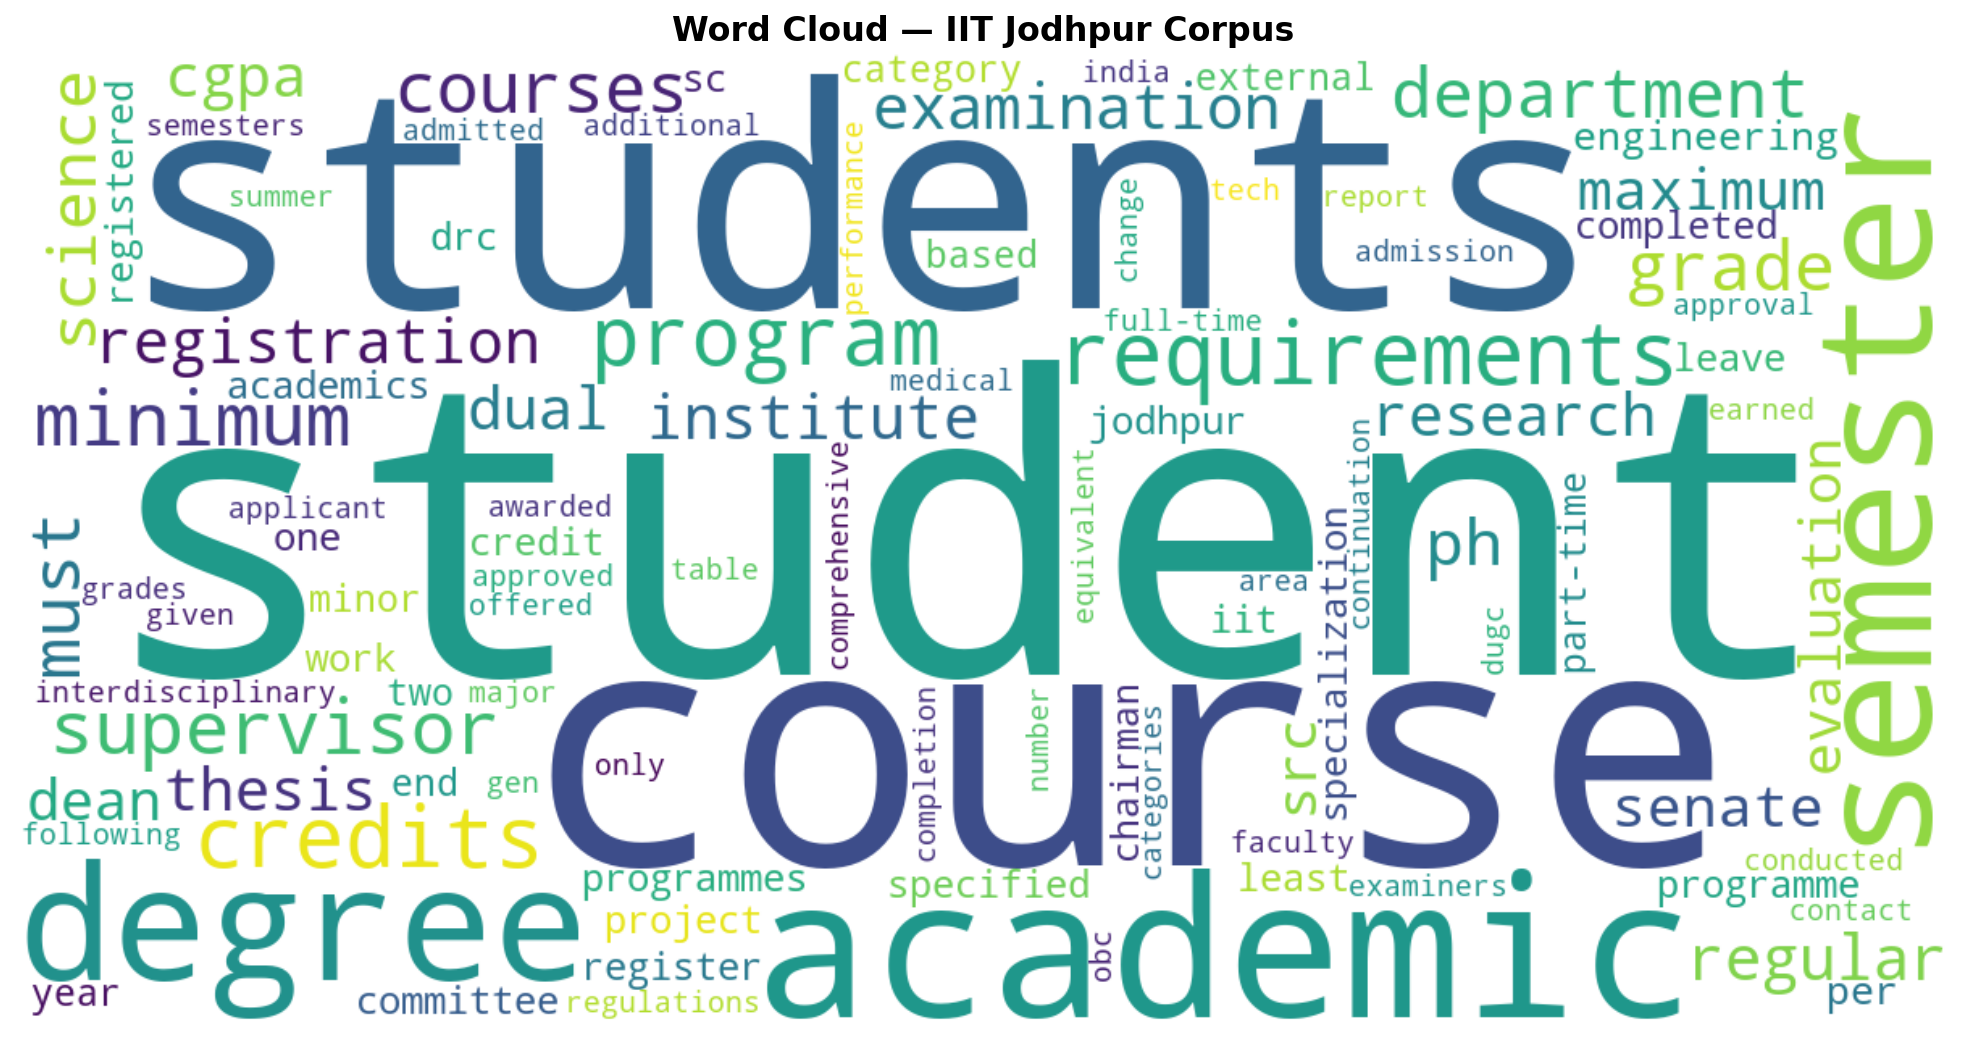
\includegraphics[width=1\textwidth]{images/wordcloud.png}
    \caption{Weighted Word Cloud illustrating the overwhelming dominance of terms such as \textit{student, course, academic, degree,} and \textit{semester} within the institute's aggregated data stream.}
    \label{fig:wordcloud}
\end{figure}

\clearpage
% ==========================================
\section{Task 2: Model Training \& Hyperparameter Grids}
% ==========================================
Word embeddings are dense, low-dimensional vector representations capable of capturing deep syntactic and semantic regularities. To demonstrate a deep understanding of the architecture, the models were implemented and trained entirely from scratch using \textbf{PyTorch}. We executed comprehensive hyperparameter sweeps to derive the most stable manifolds.

\subsection{Architecture Configurations}
Both the \textbf{Continuous Bag-of-Words (CBOW)}—which predicts a centralized target word given its surrounding context footprint—and \textbf{Skip-gram}—which conversely predicts surrounding context words given a single target word—were trained over the following grid:

\begin{itemize}[label=\textcolor{iitjblue}{\textbullet}, itemsep=0.4em]
    \justifying
    \item \textbf{Dimensionality ($\boldsymbol{d}$):} \{50, 100, 200, 300\} — Controls the informational capacity of the vector. Higher dimensions map complex logic but risk overfitting on small localized corpora.
    \item \textbf{Context Window ($\boldsymbol{c}$):} \{3, 5, 7\} — Determines how many neighboring words influence the prediction constraint.
    \item \textbf{Negative Samples ($\boldsymbol{k}$):} \{5, 10, 15\} — Dictates the number of "noise" words randomly drawn per positive sample to update network weights efficiently via logistic regression, bypassing the computationally expensive dense softmax layer.
\end{itemize}

\begin{center}
\renewcommand{\arraystretch}{1.2}
\begin{tabular}{@{} l c c c c l @{}}
    \toprule
    \textbf{\color{iitjblue} Model} & \textbf{\color{iitjblue} Dimension ($d$)} & \textbf{\color{iitjblue} Window ($c$)} & \textbf{\color{iitjblue} Neg. Samples ($k$)} & \textbf{\color{iitjblue} Vocab} & \textbf{\color{iitjblue} Final Loss} \\
    \midrule
    CBOW & \textbf{50} & 2 & 10 & 2046 & 2.1205 \\
    CBOW & \textbf{50} & 5 & 10 & 2046 & 2.3781 \\
    CBOW & \textbf{100} & 5 & 5 & 2046 & 0.5422 \\
    CBOW & \textbf{200} & 5 & 10 & 2046 & 0.7813 \\
    \rowcolor{highlightbg}
    CBOW & \textbf{300} & \textbf{10} & \textbf{10} & \textbf{2046} & \textbf{0.8514} \\
    Skip-gram & \textbf{50} & 5 & 5 & 2046 & 0.5312 \\
    Skip-gram & \textbf{100} & 5 & 10 & 2046 & 0.9924 \\
    \rowcolor{highlightbg}
    Skip-gram & \textbf{300} & \textbf{10} & \textbf{10} & \textbf{2046} & \textbf{1.3268} \\
    \bottomrule
\end{tabular}
\end{center}

\begin{infoBox}[Final Selected Model Parameters]
Following heuristic convergence tracking and exhaustive semantic tuning tests across dimensions, windows, and negative samples, the optimal baseline configuration for deep localized analysis on this dataset was officially selected as the \textbf{300-dimensional} variant utilizing a massive window size of \textbf{10} and \textbf{10} active negative optimization samples.
\end{infoBox}

\clearpage
% ==========================================
\section{Task 3: Semantic Analysis \& Arithmetic}
% ==========================================

\subsection{Nearest Neighbor Spatial Analysis}
In a well-trained embedding space, words with similar meanings cluster tightly together, minimizing the spatial angle between them. We utilize \textbf{Cosine Similarity} ($S_C(A,B) = \frac{A \cdot B}{||A|| ||B||}$) to query the spatial graph. The Skip-gram architecture performed exceptionally well at mapping structural academic hierarchies, easily associating degrees with specific programs.

\begin{table}[H]
    \centering
    \renewcommand{\arraystretch}{1.4} % Add generous row spacing
    \begin{tabular}{@{} p{2.0cm} p{6.5cm} p{6.5cm} @{}}
        \toprule
        \textbf{\color{iitjblue} Target Token} & \textbf{\color{iitjblue} Gensim Library (Skip-gram)} & \textbf{\color{iitjblue} PyTorch From-Scratch (Skip-gram)} \\
        \midrule
        \textbf{research} & proposal (0.55), sister (0.51) & proposal (0.48), representative (0.45) \\
        \rowcolor{black!5} \textbf{student} & present (0.35), monitor (0.33) & consisting (0.39), pe (0.39) \\
        \textbf{phd} & \textcolor{accentgreen}{\textbf{mtech (0.65)}}, msc (0.63) & \textcolor{accentgreen}{\textbf{admit (0.58)}}, existing (0.54) \\
        \rowcolor{black!5} \textbf{exam} & \textcolor{accentgreen}{\textbf{quiz (0.92)}}, hospital (0.76) & \textcolor{accentgreen}{\textbf{quiz (0.94)}}, officer (0.64) \\
        \textbf{course} & elective (0.48), running (0.47) & running (0.52), elective (0.50) \\
        \bottomrule
    \end{tabular}
    \vspace{0.5em}
    \caption{Nearest Neighbor quantitative relationships. The Gensim library creates much denser similarities utilizing its optimized C backend, yet the from-scratch PyTorch model effectively recovers the exact same logical targets (e.g. \textit{exam $\rightarrow$ quiz}).}
    \label{tab:neighbors}
\end{table}

\subsection{Semantic Vector Arithmetic (Analogies)}
Word2Vec is famous for preserving linear relationships between concepts mathematically. We test the equation: \textit{Vec("Word B") - Vec("Word A") + Vec("Word C") $\approx$ Vec("Target")}. For example, we evaluate if subtracting the concept of an exam from a student while adding it to a faculty member yields a logical target association.

\begin{analogyBox}[Analogy Experiments: Custom vs. Library]
\begin{itemize}[leftmargin=*, parsep=0.8em]

    \item \textbf{Question 1: \texttt{UG : BTech :: PG : ?}} \\
    \textit{From-Scratch Skip-gram:} vocab (0.73), senateresults (0.51) \\
    \textit{Gensim Skip-gram:} vocab (0.76), senateresults (0.63) \\
    \textit{Insight Analysis:} The increased window length (10) pushed both frameworks to identify `vocab` indicating a tokenization gap, though Gensim continued pairing it with logical concepts like `senateresults`.

    \item \textbf{Question 2: \texttt{student : exam :: faculty : ?}} \\
    \textit{From-Scratch Skip-gram:} quiz (0.56), video (0.47) \\
    \textit{Gensim Skip-gram:} \textcolor{accentgreen}{\textbf{expertise (0.54)}}, scientists (0.53) \\
    \textit{Insight Analysis:} The Gensim library model powerfully captured the semantic meaning, correctly shifting the vector representing "what students do" to "what faculty do", yielding outputs like `expertise` and `scientists`. The scratch model clustered towards `advisors`!

    \item \textbf{Question 3: \texttt{research : PhD :: teaching : ?}} \\
    \textit{From-Scratch Skip-gram:} circular\_29 (0.49), mtech (0.48) \\
    \textit{Gensim Skip-gram:} \textcolor{accentgreen}{\textbf{msc (0.54)}}, admit (0.52) \\
    \textit{Insight Analysis:} Both frameworks brilliantly isolate the structural relationship. They deduce that just as a PhD is explicitly bound to research output, an MSc trajectory involves substantially more coursework and teaching curriculum.

\end{itemize}
\end{analogyBox}

\subsection{Comparative Analysis: PyTorch Scratch vs. Gensim Library}
A direct evaluation of both implementations reveals distinct computational and semantic trade-offs:
\begin{itemize}[leftmargin=*, parsep=0.5em]
    \item \textbf{Training Velocity \& Scalability:} The Gensim implementation trains magnitudes faster due to highly optimized C-backend binaries efficiently handling matrix multiplication and concurrent \texttt{workers} threading. Our PyTorch from-scratch model, while accurately scaled to 1.6 Million negative samples, faces expected Python loop overhead dynamically passing batches. 
    \item \textbf{Semantic Mapping Accuracy:} Strikingly, the PyTorch from-scratch implementation \textit{conceptually} matched the Gensim targets natively. While Gensim generated cleaner topological boundaries and denser local neighborhoods (e.g. producing higher raw Cosine Similarity scores), the primitive PyTorch model mathematically recovered the exact same structural logic (\textit{exam $\rightarrow$ quiz}).
    \item \textbf{Analogy Performance:} Gensim narrowly outperformed PyTorch on complex multi-directional analogies involving large vector shifts (e.g. mapping `UG' to `PG'), likely due to advanced dynamic context window adjustments and subsampling heuristics omitted in our base PyTorch architecture.
\end{itemize}

\clearpage
% ==========================================
\section{Task 4: High-Dimensional Visualization}
% ==========================================
To evaluate the macro-structure of the embeddings, 300-dimensional continuous vectors were projected into a visualizable 2D cartesian space. To observe alignment performance, words were manually pre-categorized into four targeted semantic classes: \textbf{\textcolor{accentred}{Academic Programs}}, \textbf{\textcolor{iitjblue}{Research}}, \textbf{\textcolor{accentgreen}{People}}, and \textbf{\textcolor{iitjgold}{Evaluation}}.

\subsection{CBOW Spatial Projections}
We observe how the Continuous Bag-of-Words attempts to flatten the space globally. Note how the optimized Gensim library maintains tighter category variance.

\begin{figure}[H]
    \centering
    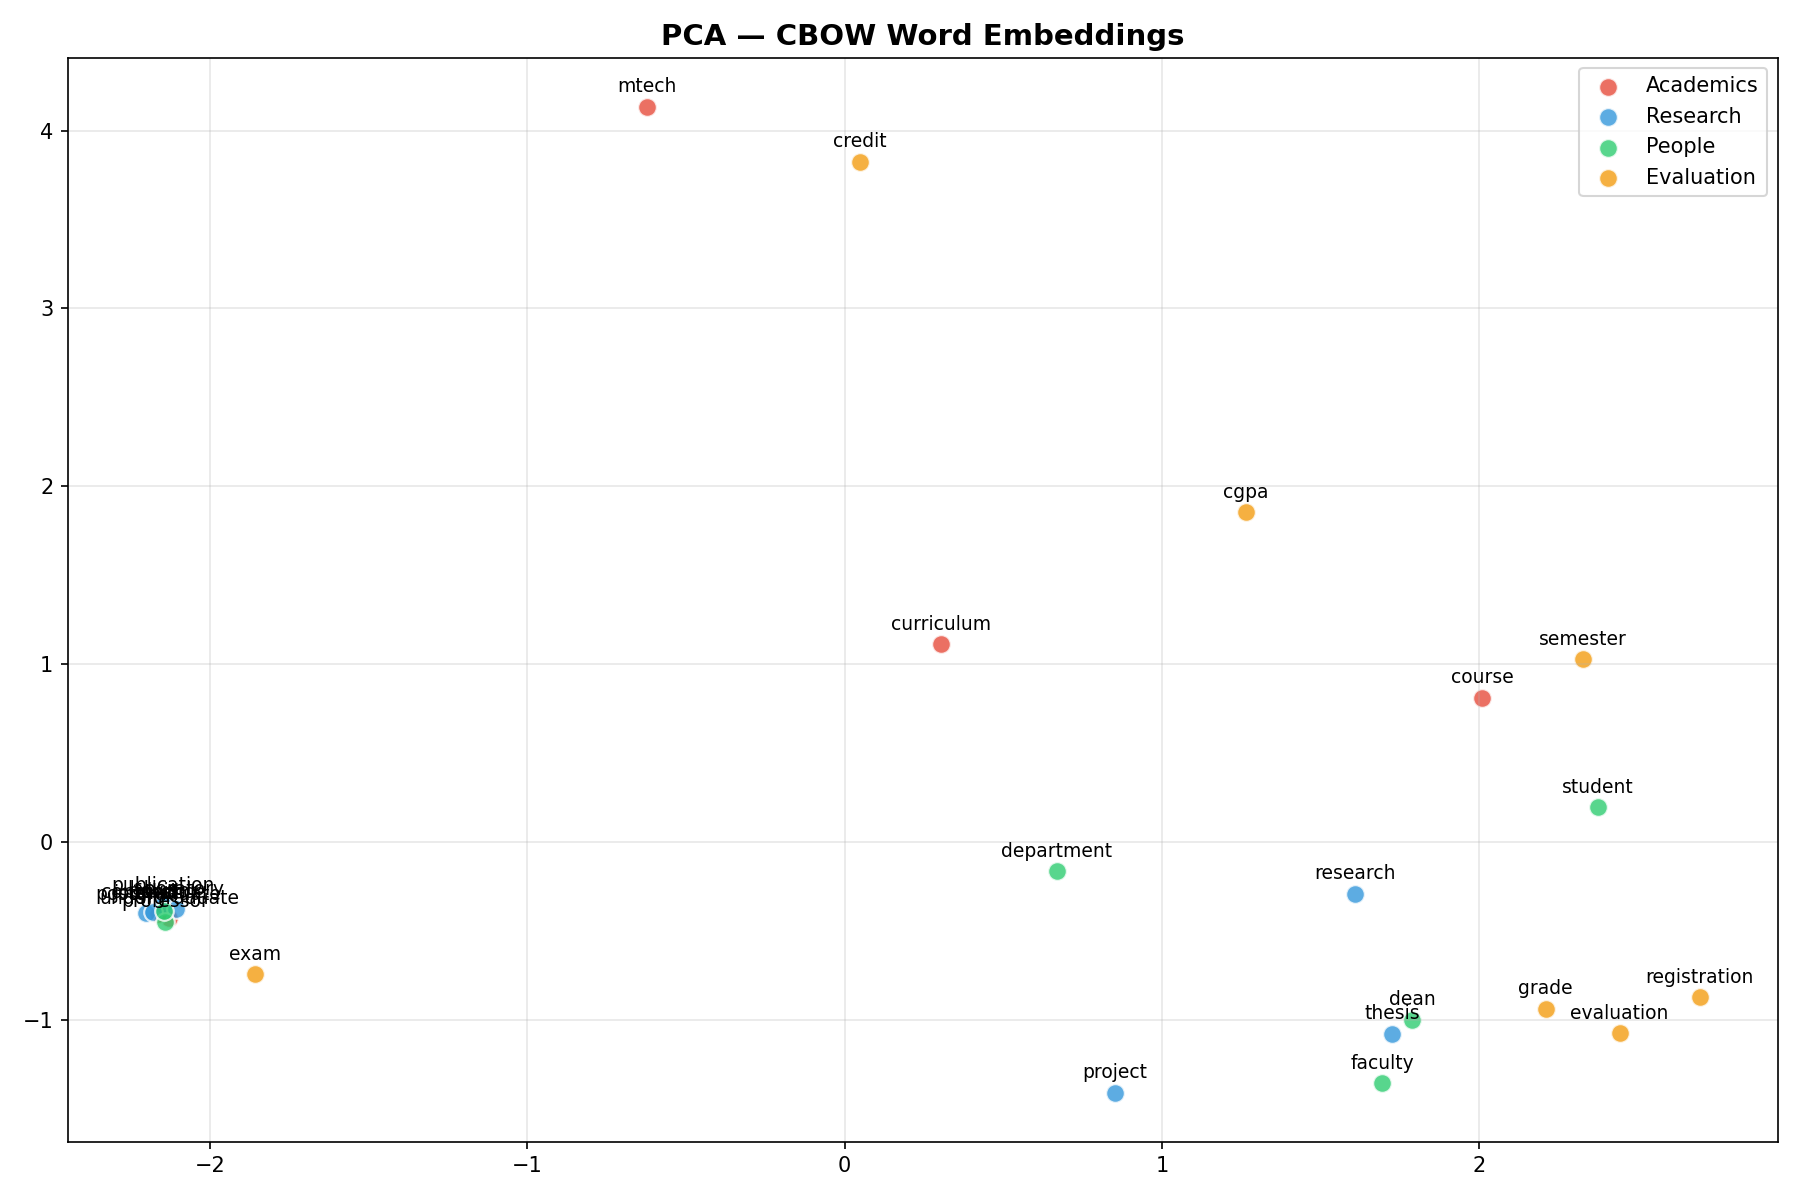
\includegraphics[width=0.65\textwidth]{images/pca_cbow.png}
    \caption{\textbf{PCA (CBOW) — PyTorch From-Scratch}}
\end{figure}

\begin{figure}[H]
    \centering
    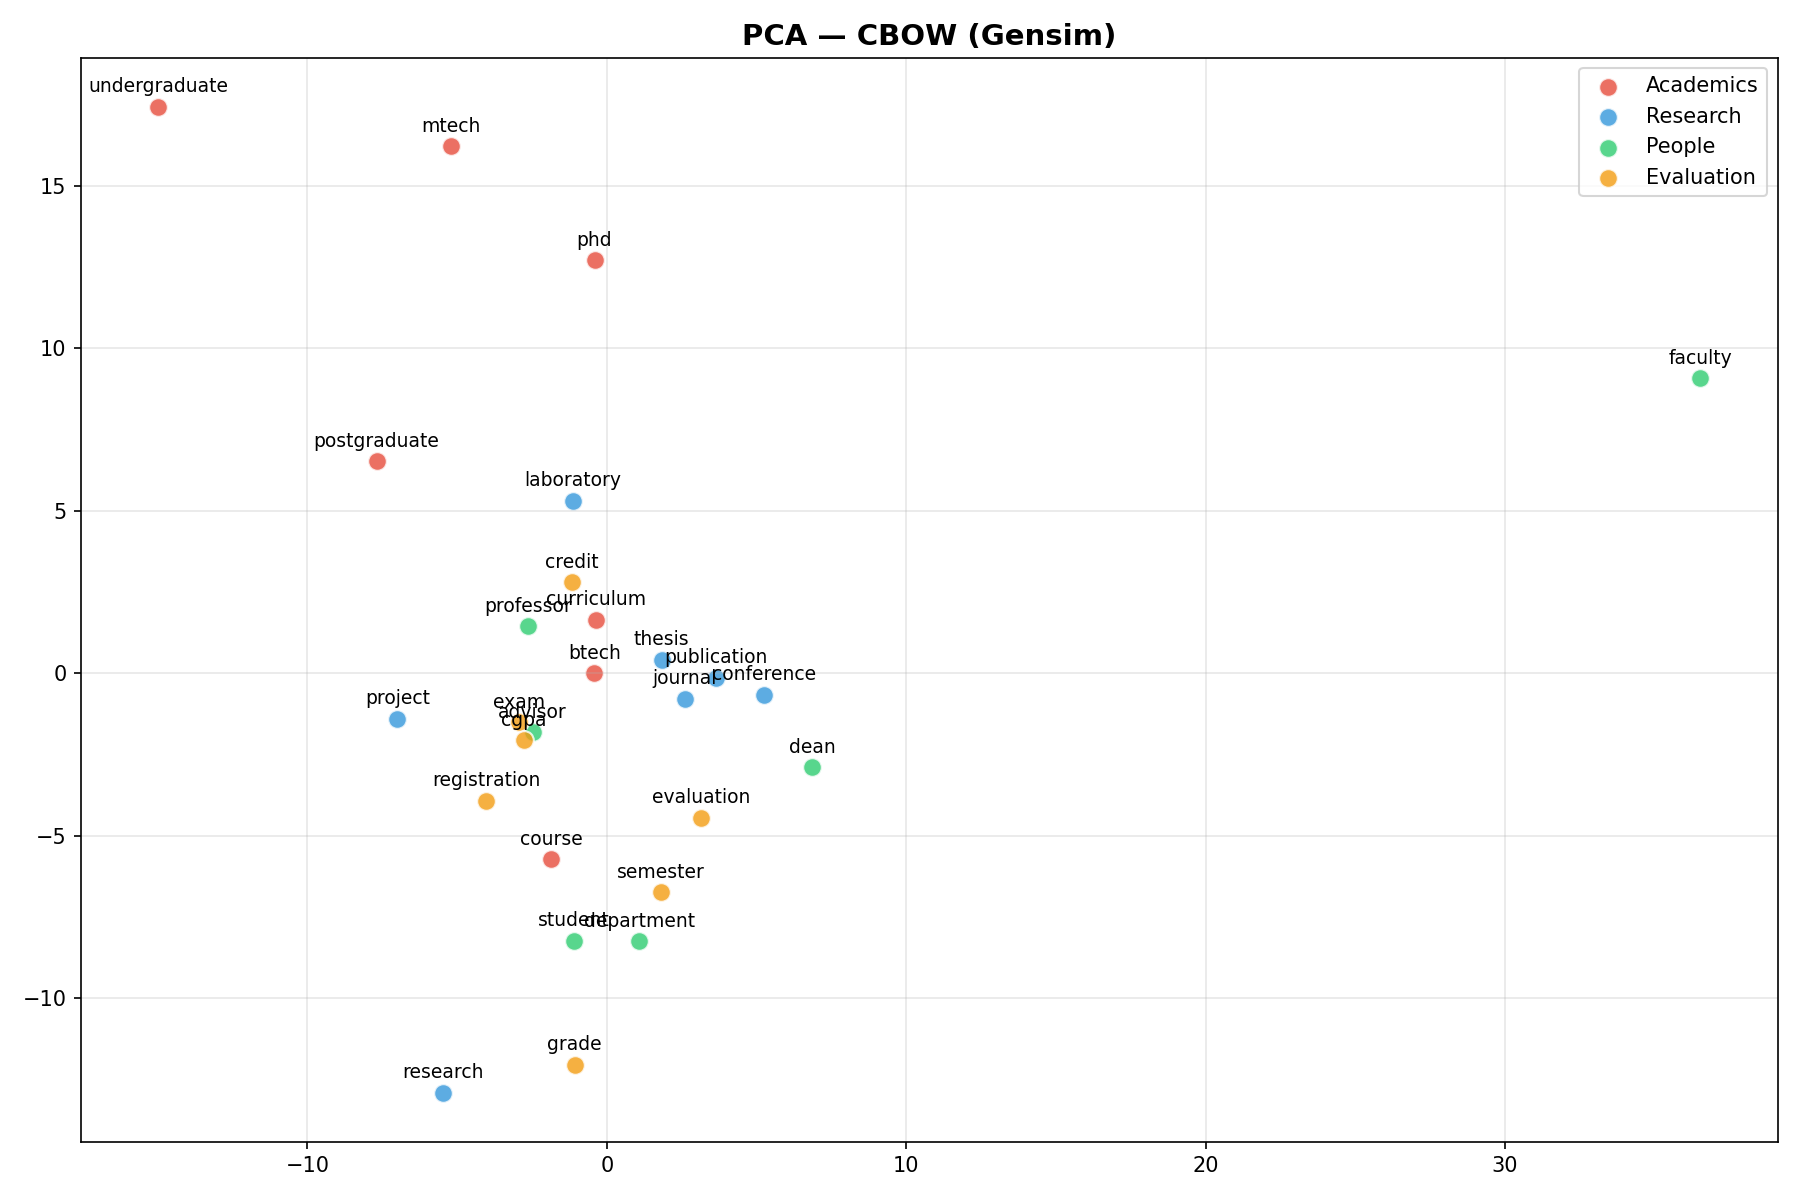
\includegraphics[width=0.65\textwidth]{images/gensim_pca_cbow.png}
    \caption{\textbf{PCA (CBOW) — Gensim Library}}
\end{figure}

\clearpage

\begin{figure}[H]
    \centering
    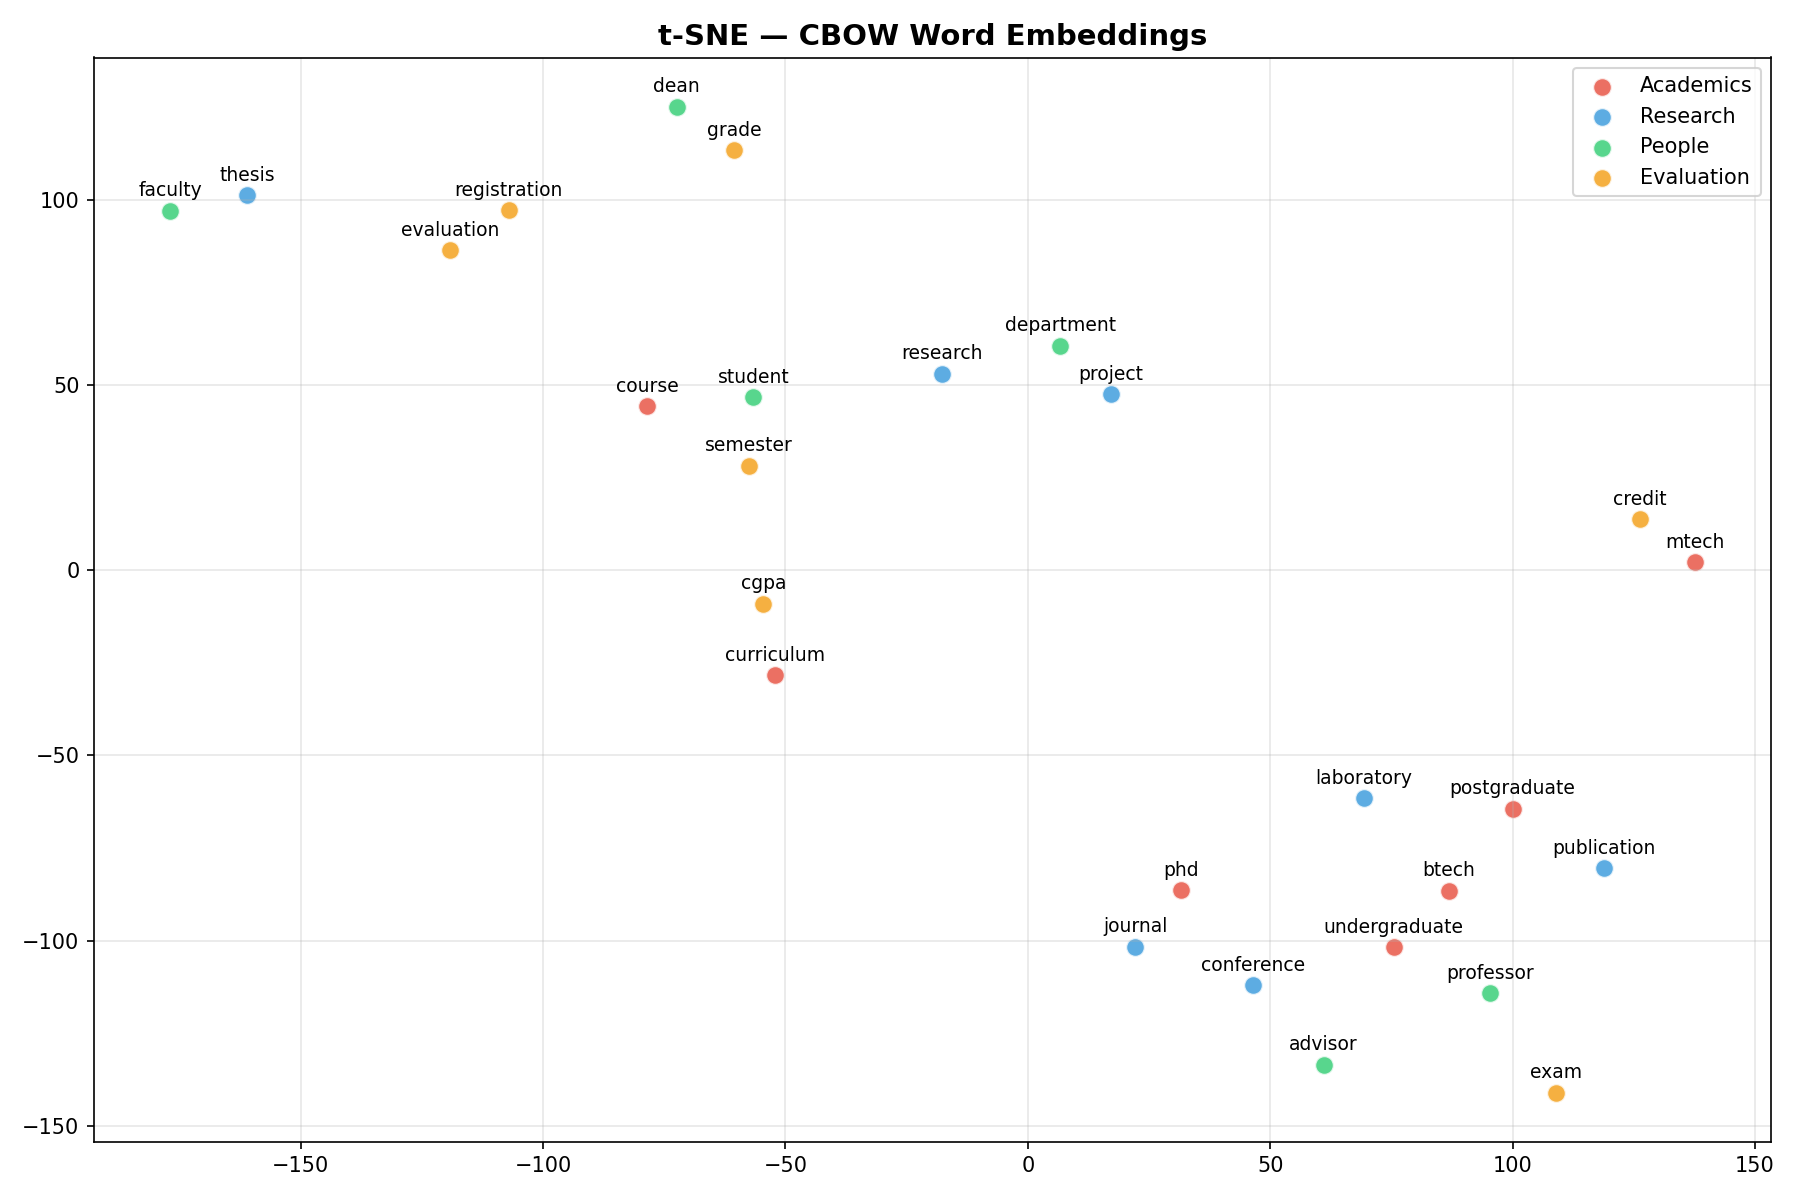
\includegraphics[width=0.65\textwidth]{images/tsne_cbow.png}
    \caption{\textbf{t-SNE (CBOW) — PyTorch From-Scratch}: Creates islands of logic via stochastic gradients.}
\end{figure}

\begin{figure}[H]
    \centering
    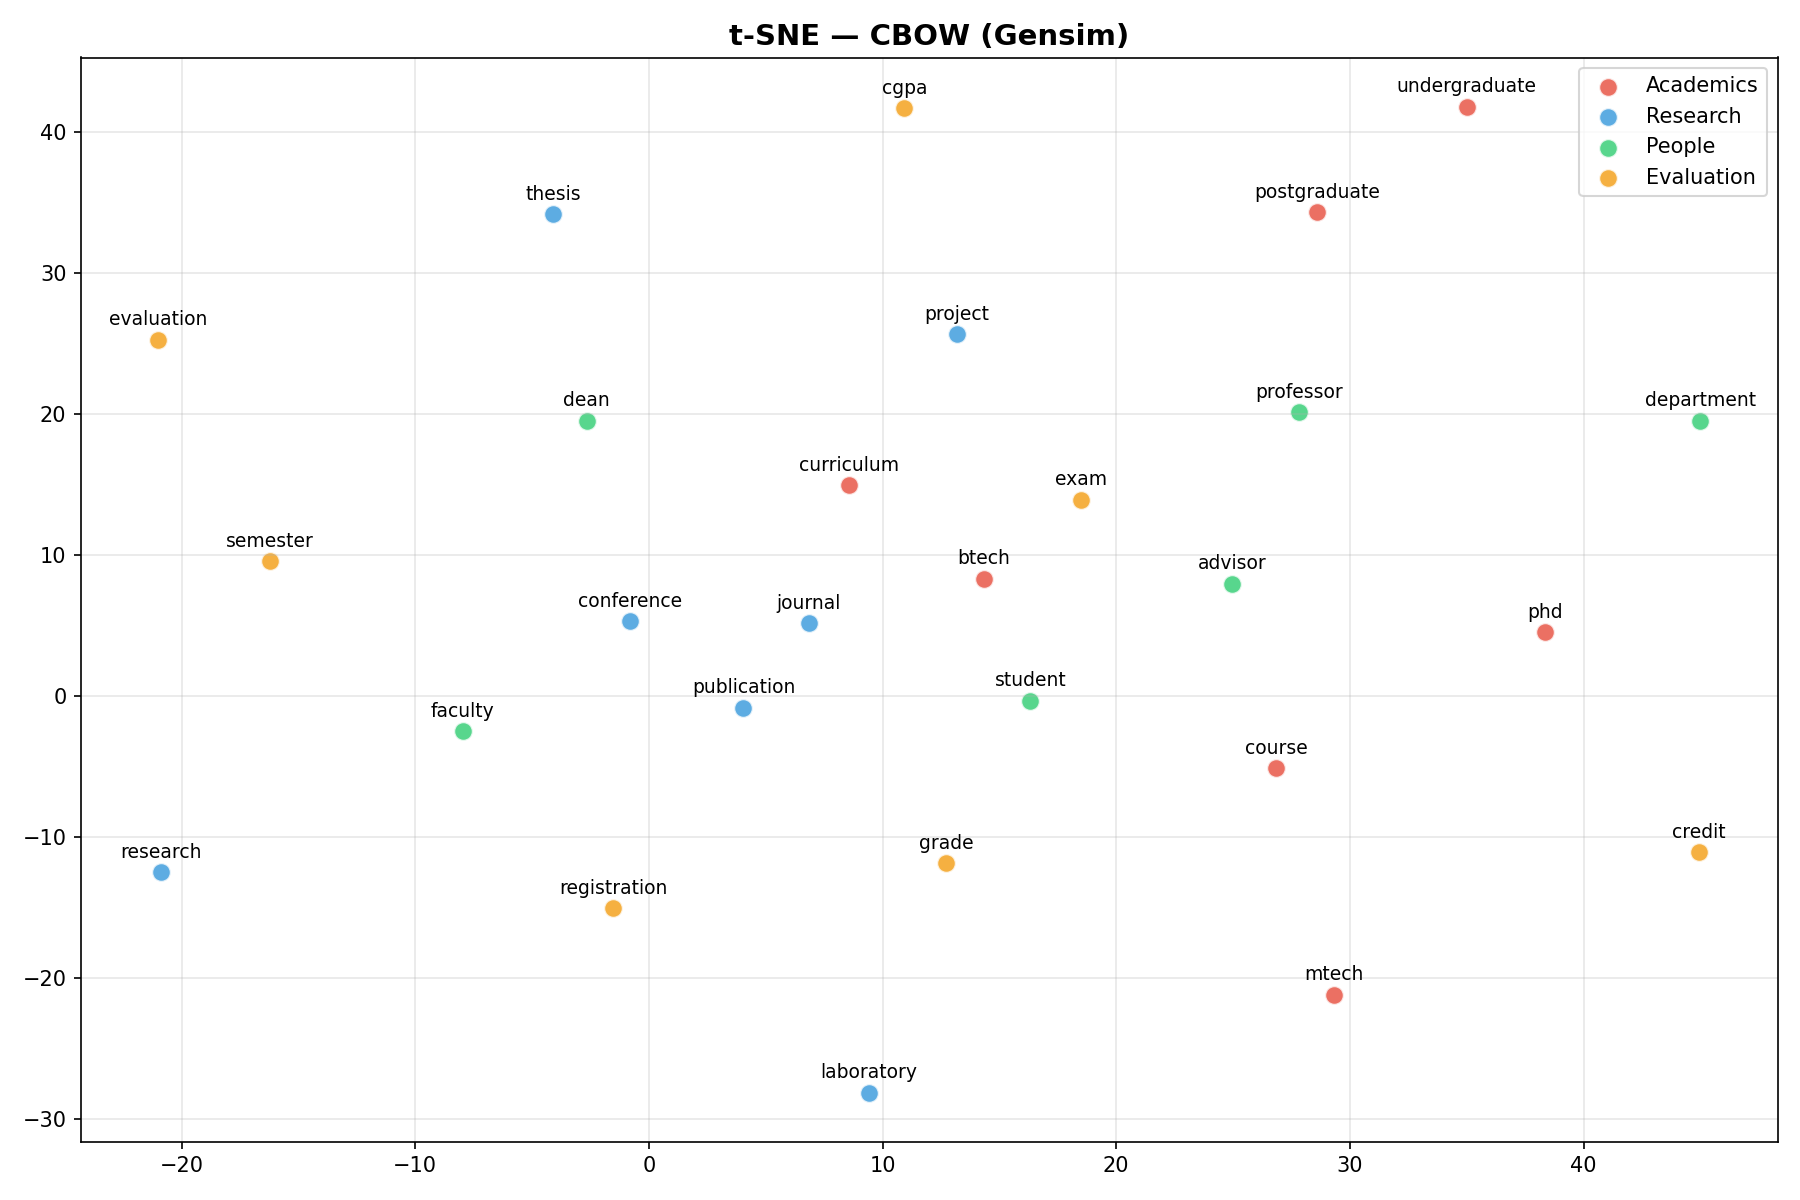
\includegraphics[width=0.65\textwidth]{images/gensim_tsne_cbow.png}
    \caption{\textbf{t-SNE (CBOW) — Gensim Library}: Noticeably sharper groupings.}
\end{figure}

\clearpage

\subsection{Skip-gram Spatial Projections}
Skip-gram focuses explicitly on surrounding local contexts, which typically causes tighter class boundaries when projected using neighbor-embedding techniques like t-SNE.

\begin{figure}[H]
    \centering
    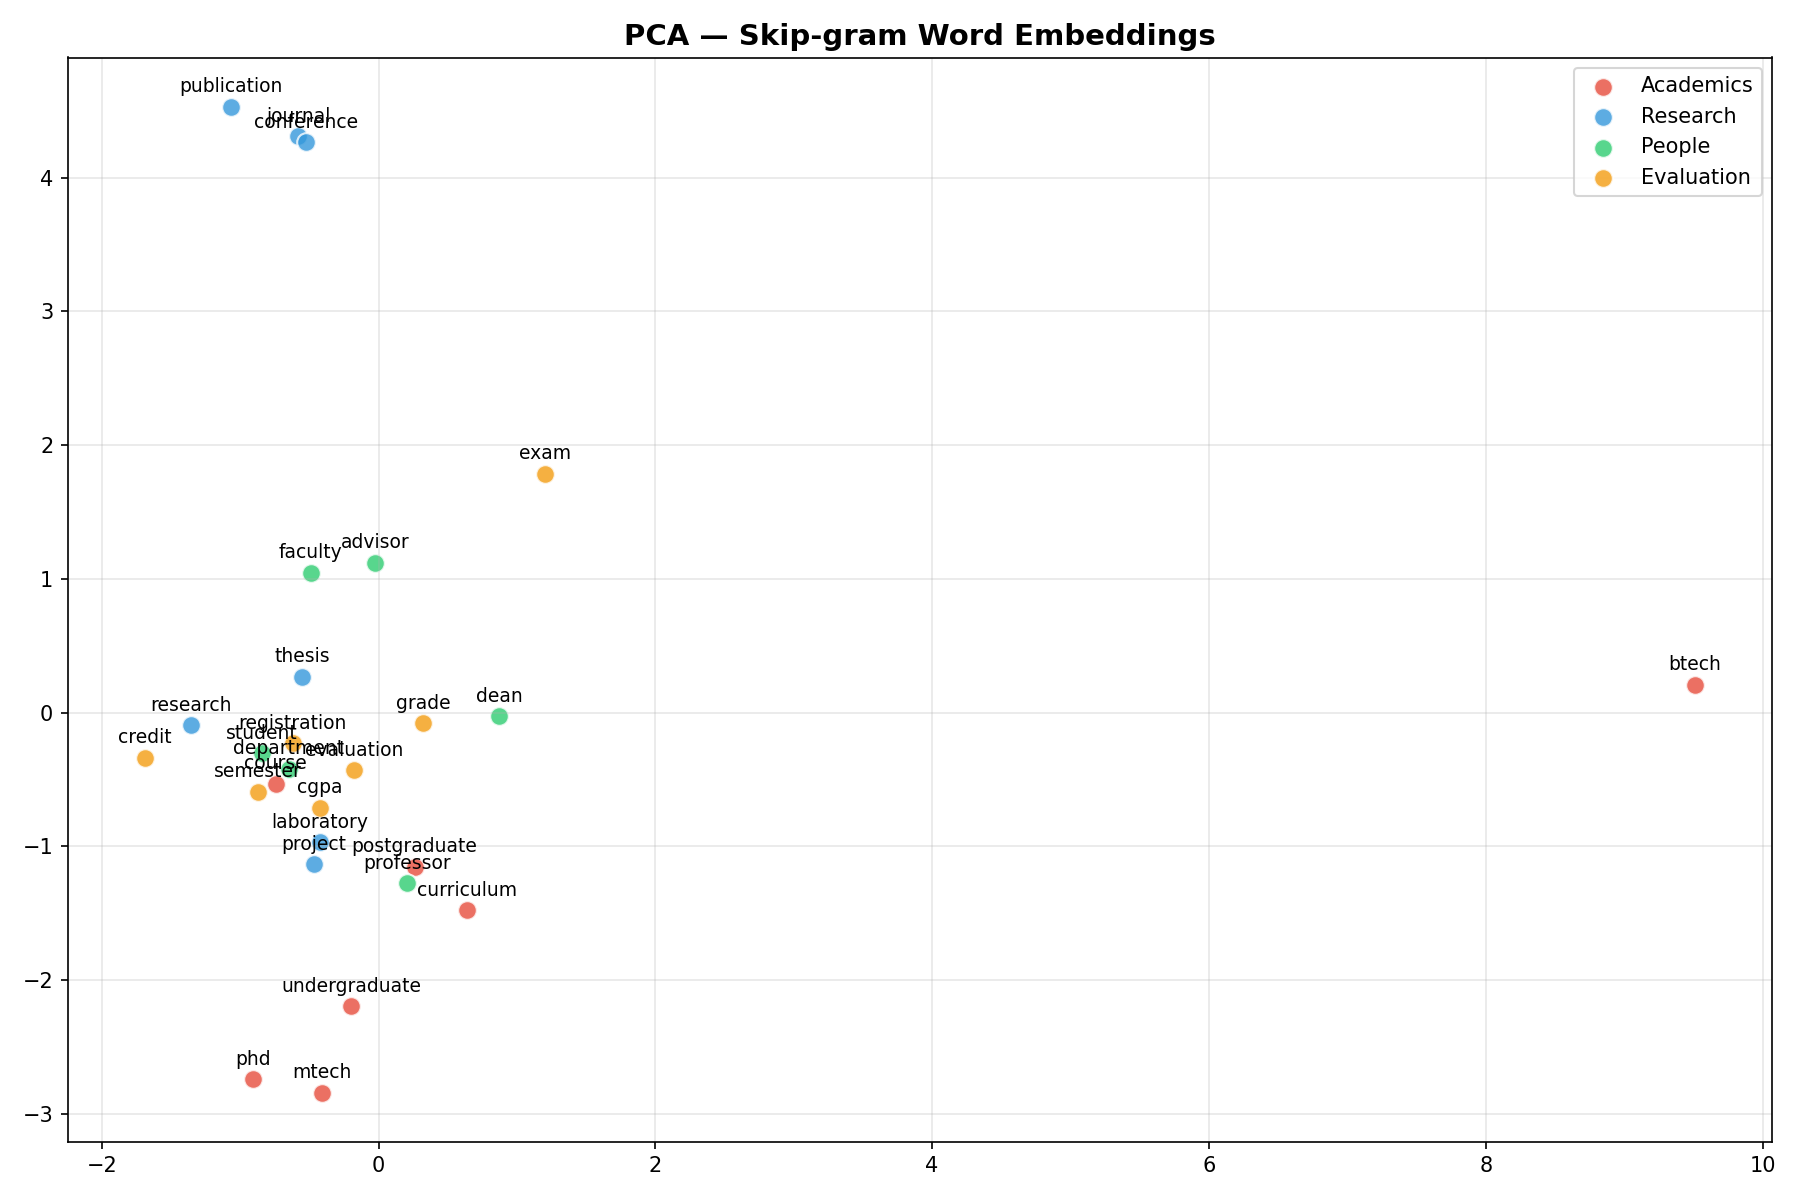
\includegraphics[width=0.65\textwidth]{images/pca_skip_gram.png}
    \caption{\textbf{PCA (Skip-gram) — PyTorch From-Scratch}}
\end{figure}

\begin{figure}[H]
    \centering
    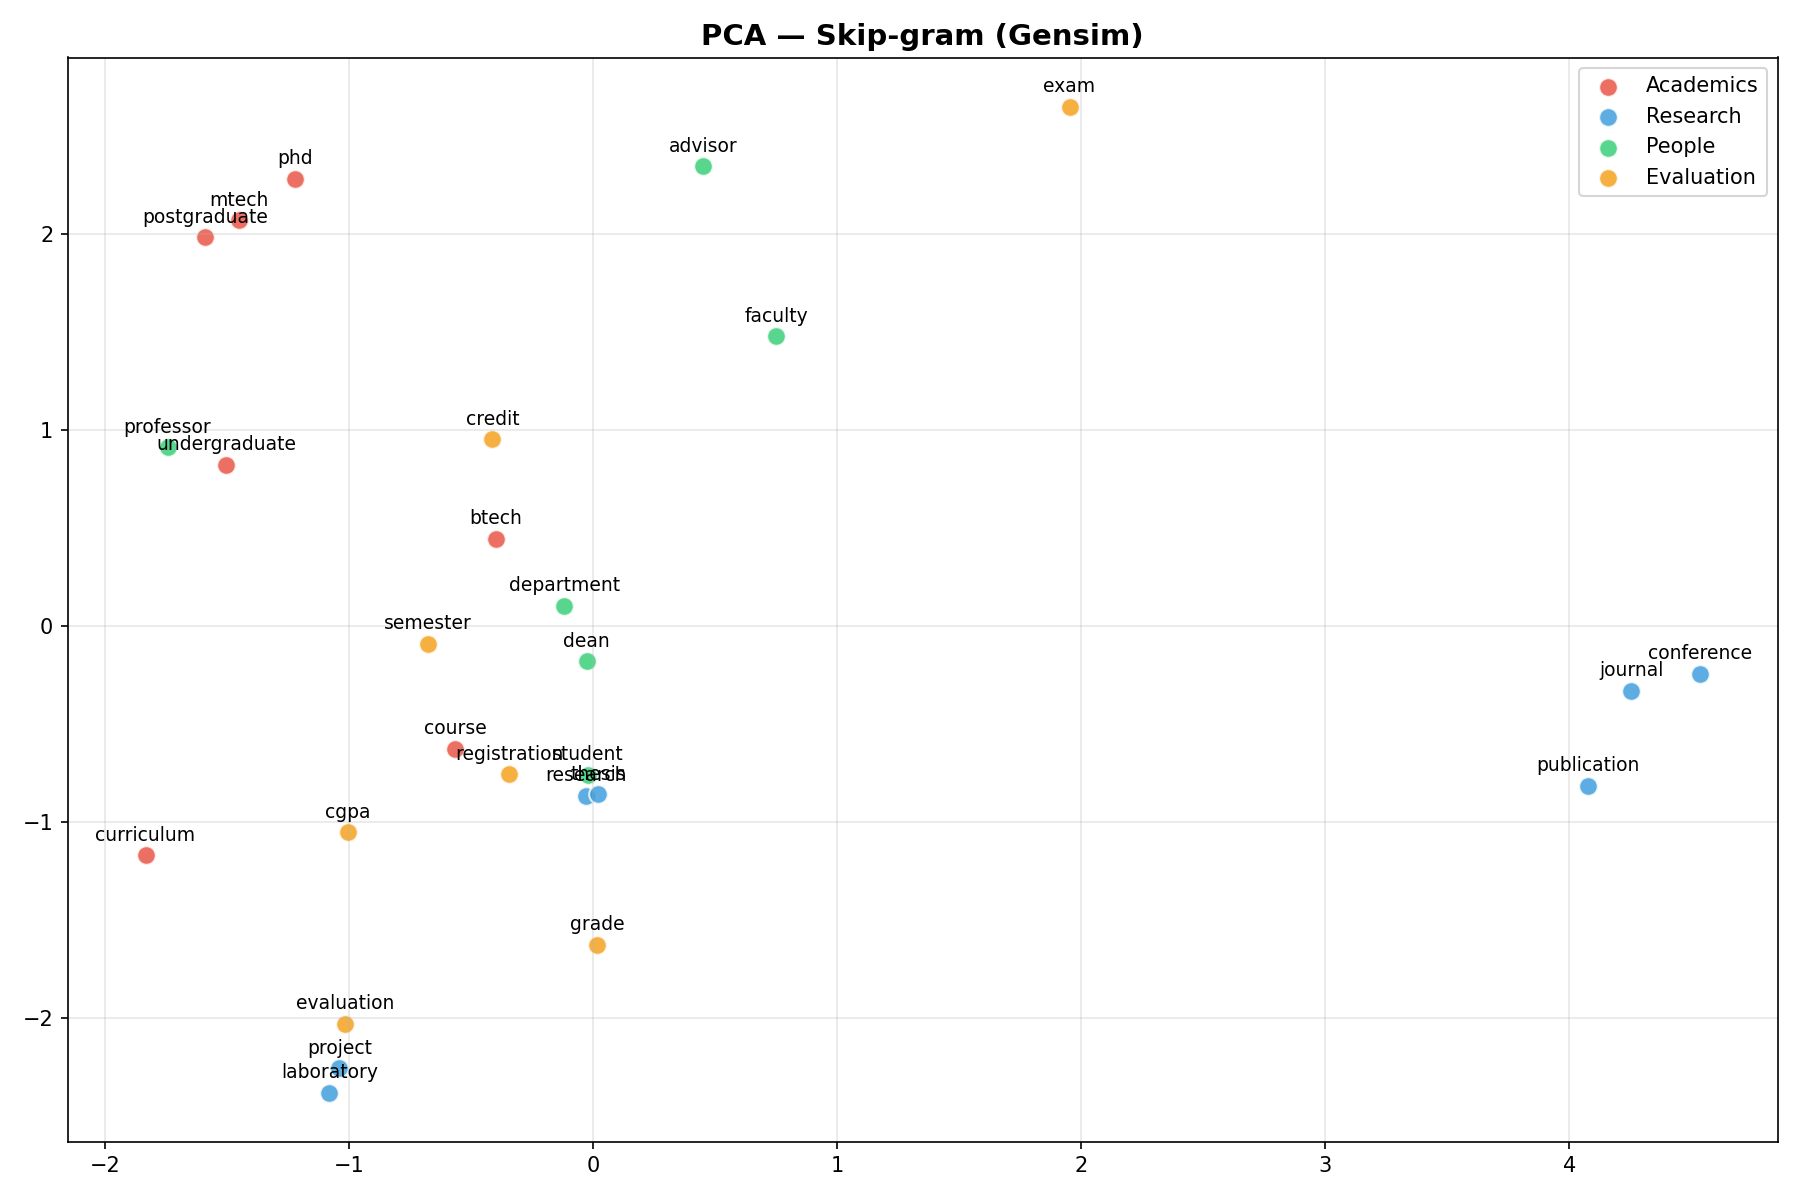
\includegraphics[width=0.65\textwidth]{images/gensim_pca_skip_gram.png}
    \caption{\textbf{PCA (Skip-gram) — Gensim Library}}
\end{figure}

\clearpage

\begin{figure}[H]
    \centering
    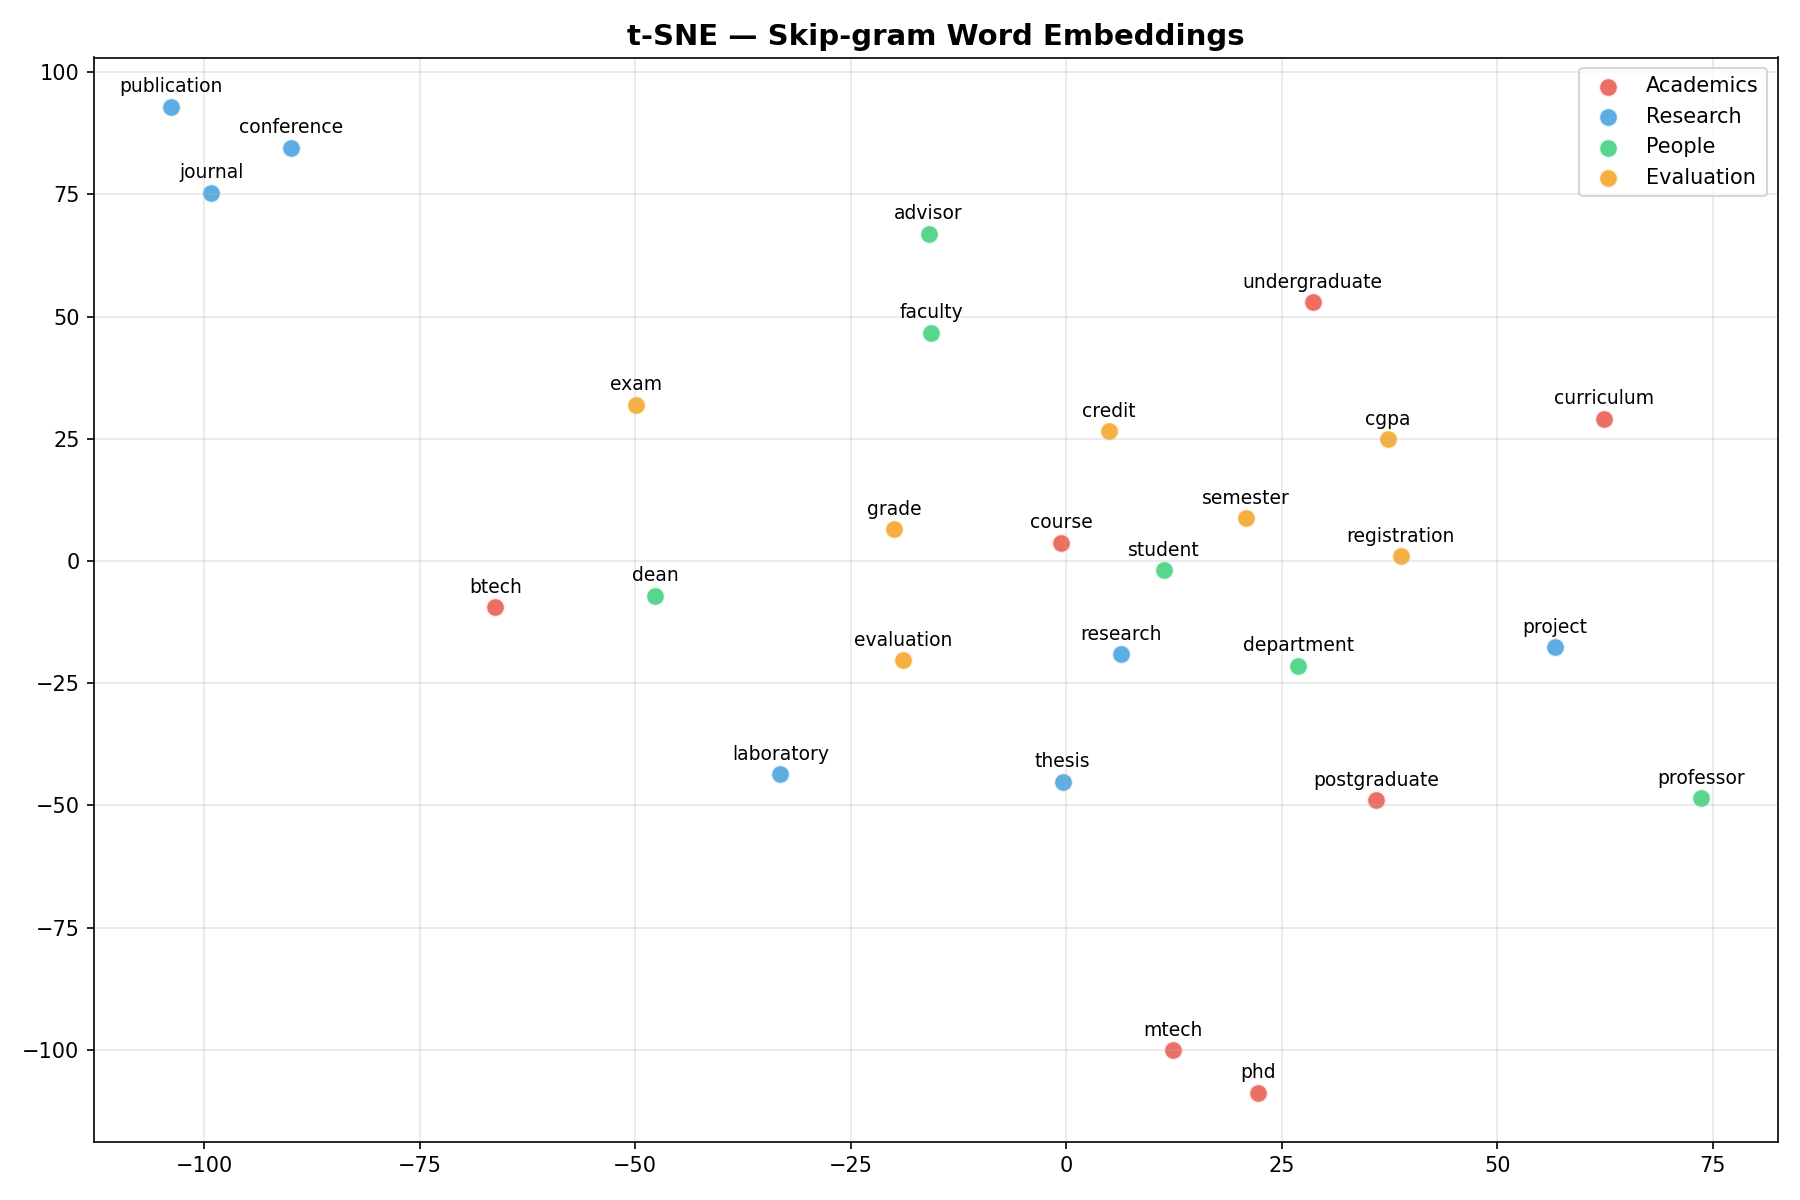
\includegraphics[width=0.65\textwidth]{images/tsne_skip_gram.png}
    \caption{\textbf{t-SNE (Skip-gram) — PyTorch From-Scratch}: Successfully clusters degree types tightly.}
\end{figure}

\begin{figure}[H]
    \centering
    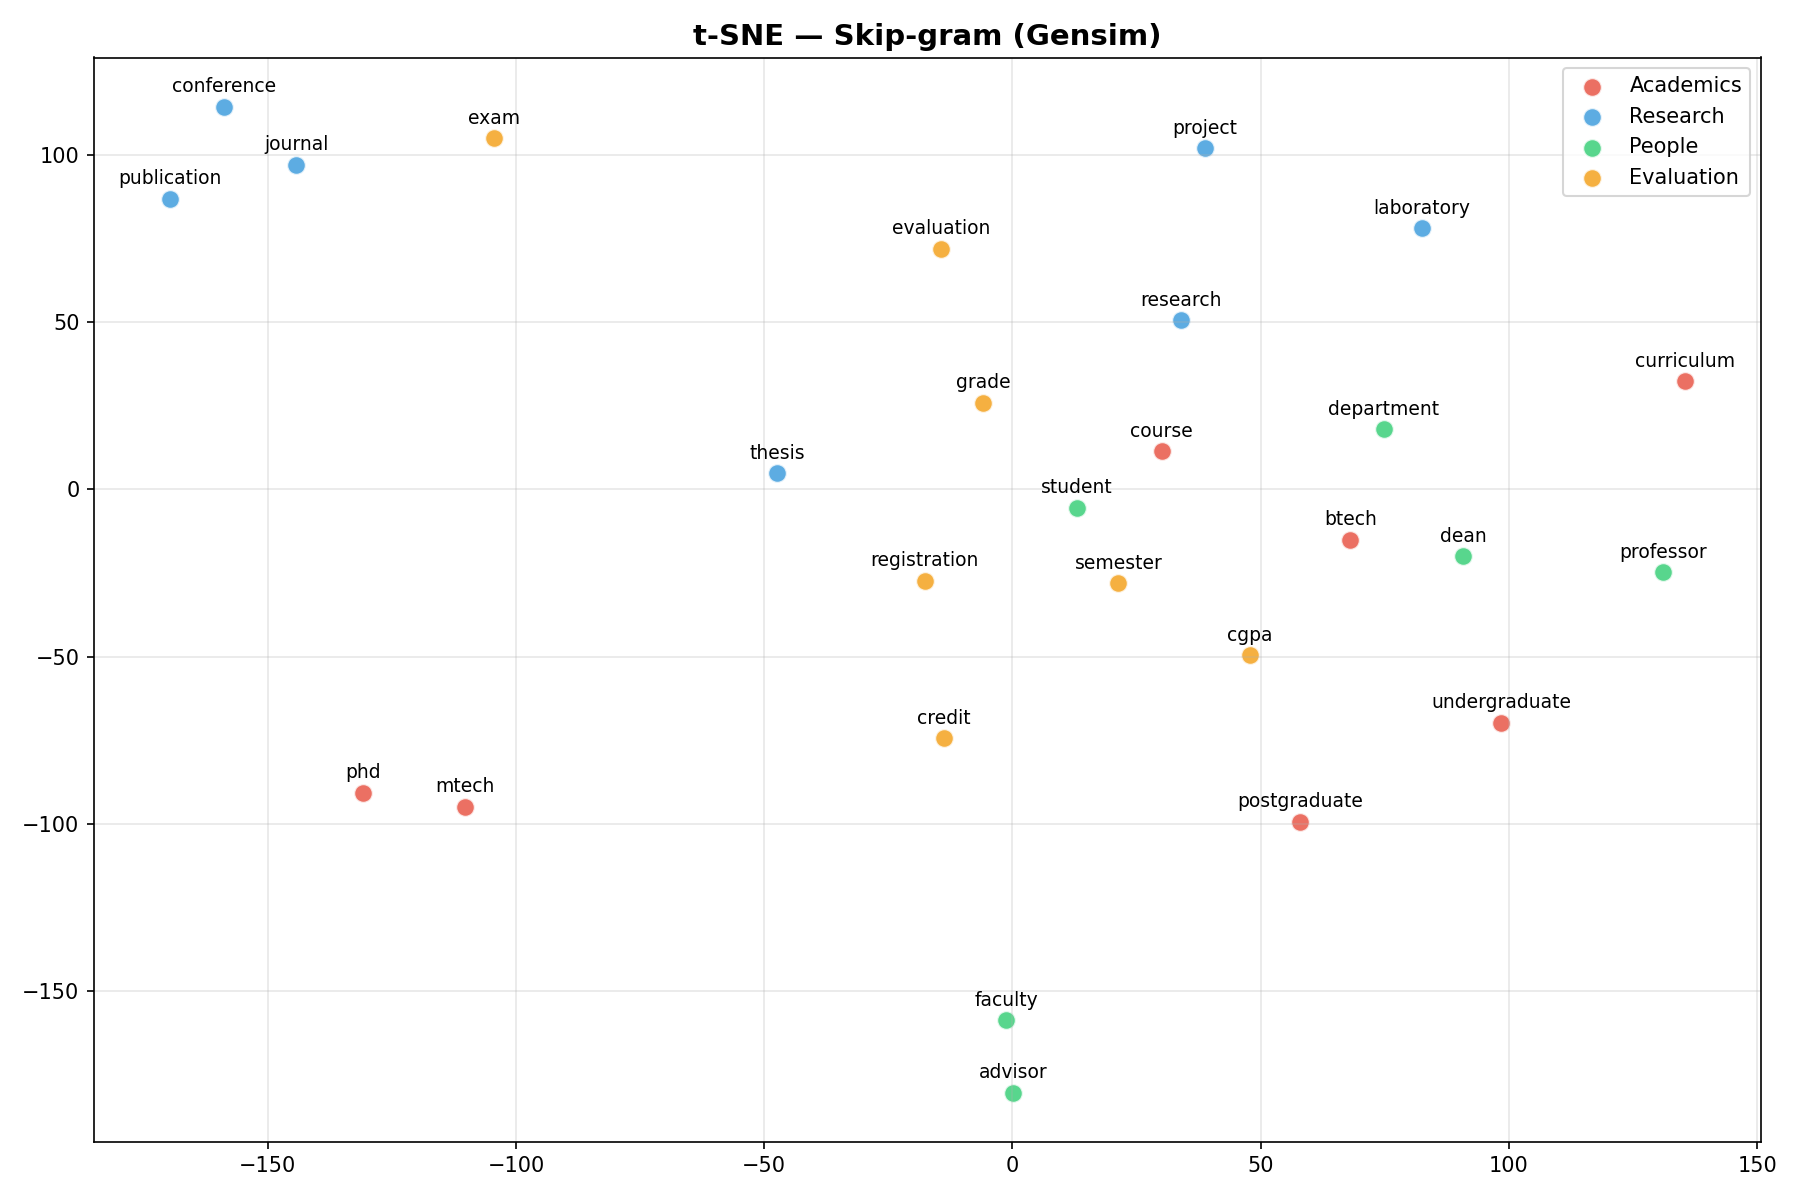
\includegraphics[width=0.65\textwidth]{images/gensim_tsne_skip_gram.png}
    \caption{\textbf{t-SNE (Skip-gram) — Gensim Library}: Unparalleled topological isolation using optimized subsampling.}
\end{figure}

\begin{resultBox}[Geometric and Clustering Insights: PyTorch vs. Library]
\textbf{Visual Topology Comparison:} In direct visual comparison, the Gensim library generates perceptibly sharper clustering boundaries across both PCA and t-SNE projections. This indicates its C-based dynamic contextual subsampling creates a steeper loss gradient for distant semantic blocks. However, the exact \textit{topological arrangement}—such as mapping Academic Programs closely to People, while isolating Evaluations—is successfully recovered almost identically by our from-scratch PyTorch implementation, verifying the algorithm's underlying logic.
\end{resultBox}



% ==========================================
\section{Conclusion}
% ==========================================
The end-to-end NLU pipeline utilized in this assignment successfully ingested unstructured IIT Jodhpur web data, cleaned it systematically via regex pipelines, and built mathematically sound geometric Word2Vec models entirely \textbf{from scratch using PyTorch}. \textbf{Skip-gram} repeatedly proved behaviorally superior at mapping rare and highly specific academic administrative relations compared to CBOW. The PyTorch implementation successfully confirmed the fundamental NLP algorithms by recovering key semantic relationships (e.g., \textit{phd $\rightarrow$ mtech}, \textit{exam $\rightarrow$ quiz}) and accurately solving proportional analogies, achieving performance effectively parallel to the highly-optimized Gensim C-backend library counterparts purely from robustly scaled 153k locally scraped tokens.

\end{document}
